\subsection*{Optimisation/Runtime Efficiency}
As code is generated considerations of efficiency can be made such that the object code becomes more efficient than other alternatives.
Rather than blindly translating the source code, translating to something more efficient is a subproblem in compiler optimisation.
Optimisation is however nonspecific and subjective, for \gls{gamble} we will instead be referring to runtime efficiency.
Runtime efficiency entails considerations of memory allocation, pipelining, parallelisation and others that may have an impact on execution time.
To do an efficient and complete analysis of how to increase runtime efficiency, information of the situation in program is required.
This is where \gls{gamble} is at a disadvantage. 
\gls{gamble} distances its programmers from controlling where the code is performed and instead does so seamlessly.
Information about how e.g. a for-loop could be transformed into a kernel does not exist in \gls{gamble} which makes it difficult to do this.
The seamless use of the \acrshort{gpu} means that information is lackluster and therefore all computations may not available candidates for improving upon runtime efficiency, this is one of the tradeoffs \gls{gamble} makes.
If \gls{gamble} were to require more information, e.g. whether or not something is parallelisable or ask the programmer to determine what memory should be used for each variable, the simplicity and seamless use of the \acrshort{gpu} would be lost.

As previously mentioned due the object code being OpenCL C certain considerations pertaining to instruction handling and register allocation etc. are not of interest for this compiler.
Instead to increase runtime efficiency the considerations instead pertain to when the \acrshort{gpu} should be used, the generated C code as well as the OpenCL kernels.

As \gls{gamble} is attempting to seamlessly use the \acrshort{gpu} to increase performance, knowing when the use of the \acrshort{gpu} will actually be beneficial is an important point in the code generation process.
As mentioned to do this efficiently, the compiler would require more information about the computations which are to be performed, than can be read from the syntax of \gls{gamble}.
Therefore the it is decided that it is better to be sure that a computation can benefit from the \acrshort{gpu}, rather than risking moving computations that wont benefit with those that will.
As such only those operations that the project group knows have a possibility of benefiting from the parallel abilities of the \acrshort{gpu} will be executed on the \acrshort{gpu}.

%Knowing when to use GPU
Even though a computation can be parallelised, does not necessarily mean it should be moved to the \acrshort{gpu}, as is evident in \myref{image:benchmark}.
This is an opportune moment for improving the runtime efficiency of the object code by using the \acrshort{gpu} only when it will be superior than the gpu in regards to performance.
A possibility of doing so would be to analyse whether or not an instruction sequence both entail a sufficient amount of operations and that these are not sequentially dependand on each other.
Performing such an analysis increases compile time and may runtime efficiency.
Because of the difficulty to discern not only if there will be an actual increase, but also if any custom functions created by the programmer are fit to run on the \acrshort{gpu} this analysis is part of the \gls{gamble} compiler.
Instead only vector and matrix operations already defined in the language will be performed on the \acrshort{gpu}.

%Optimising OpenCL Kernals
A function that is to be run on the \acrshort{gpu} is in the OpenCL framework called a kernel.
Since kernel code uses explicit memory handling, one must choose what memory space to allocate ones variables in.
In the different kernels the better one utilises its memory the faster a kernel can be executed, as a result of the memory used being located higher in the memory hierarchy.
\begin{figure}[h!]
\centering
 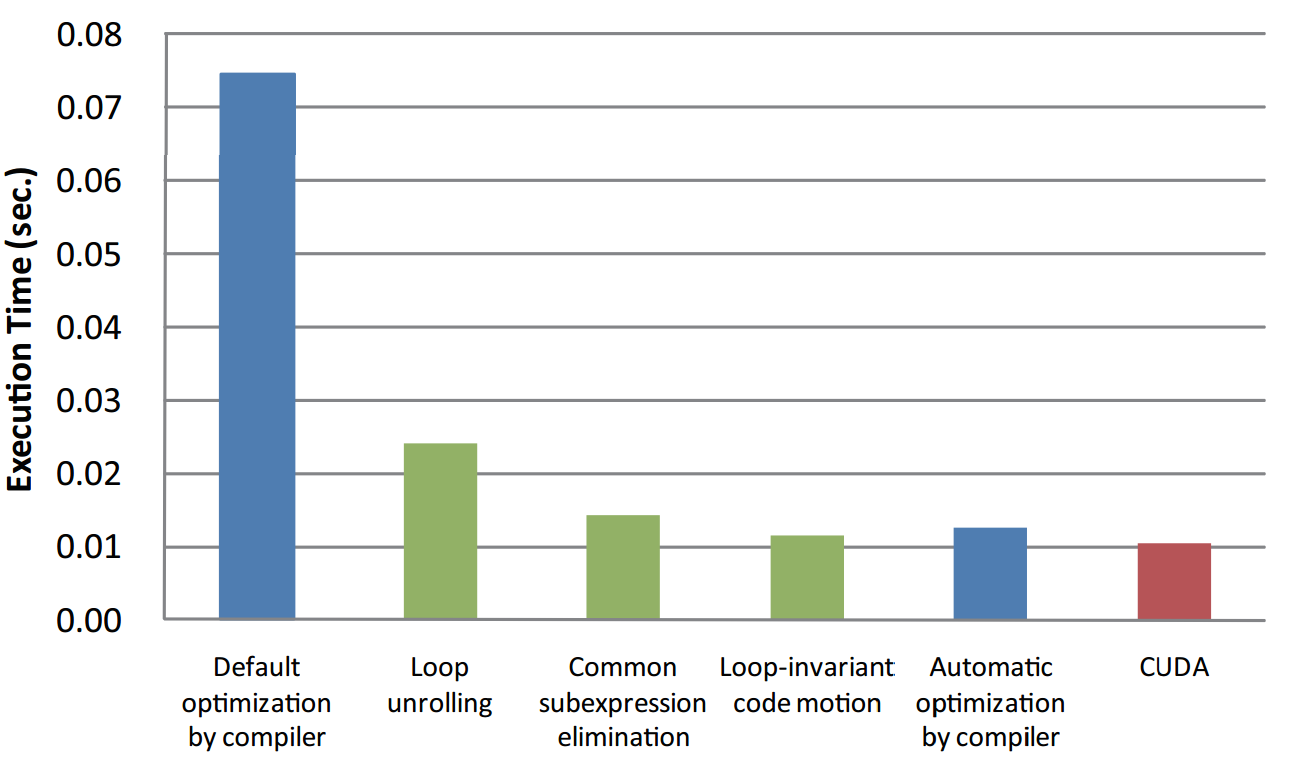
\includegraphics[width=1\textwidth]{figures/opencloptimisation.png} % trim=4.85cm 15cm 0.85cm 1cm
\caption{Execution speed of a matrix multiplication with different optimisation levels. \citep{CUDAOpenCLOptimisation}}\label{image:OpenCLOptCompare}
\vspace{-15pt}
\end{figure}
As seen on \myref{image:OpenCLOptCompare} some possible methods of increasing runtime efficiency includes loop unrolling, common sub-expression elimination and loop-invariant code motion. 
These are taken as specific examples in this comparison because these methods are performed in the \acrlong{ptx} code that CUDA compiles.
An OpenCL C compiler also provides the option of doing optimisation upon the code, however it would seem that depending on the \acrshort{gpu} and platform one is working on some methods of increasing runtime efficiency depend on the platform.
This in particular entails the ideal work-group size changes, making universal optimisation a difficult task to take on.
OpenCL uses just-in-time compilation to generate binary code to the appropriate device it is working with.
While this allows it to be used on more platforms than one like CUDA, it also results in compiler runtime efficiency improvements to significantly increase compile time and thus increases the total execution time, runtime as well as compile time.\citep{CUDAOpenCLOptimisation}

%Optimising C code(CPU)
As \gls{gamble} does not exclusively perform its operations on the \acrshort{gpu} the code run on the \acrshort{cpu} must also be considered as a point in which runtime efficiency can be increased.
Some methods of increasing runtime efficiency on the \acrshort{cpu} are similar as mentioned earlier such as loop unrolling.
Further methods pertain to the architectural differences between \acrshort{cpu}s and \acrshort{gpu}s, in particular cache- and pipeline-friendly code.
Cache-friendly code means considering the principle of spatial locality i.e. memory regions closer to each other, are more likely to be accessed within a short time.
To write pipeline-friendly code one must in particular consider branch prediction, however the best way is simply to avoid branching.\citep{CCodeOpt}
While these methods may very well increase runtime efficiency, there is no reason to implement them as the GNU Compiler Collection already implements well developed methods of increasing runtime efficiency beyond our abilities.